\section{Aufbau und Durchführung}
\label{sec:AufbauundDurchführung}
\begin{figure}[h!]
	\centering
	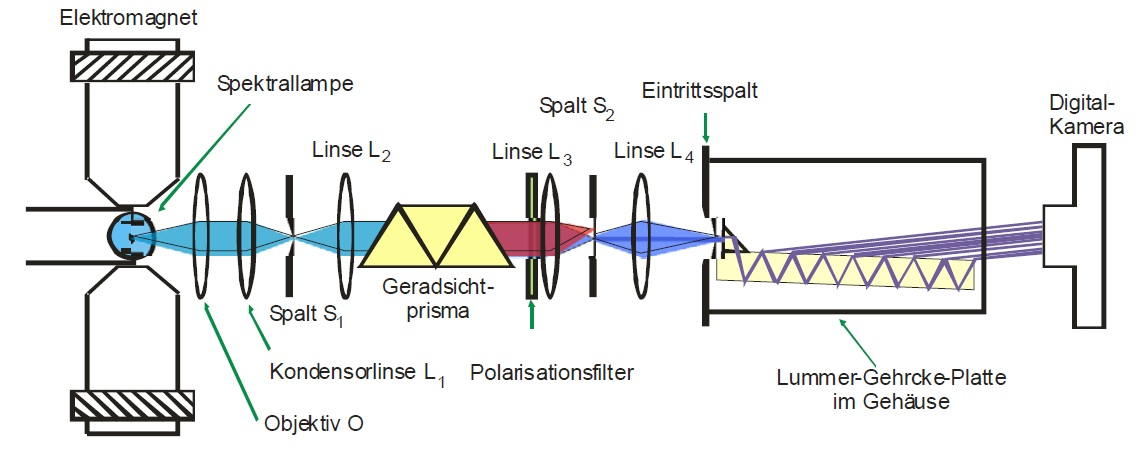
\includegraphics[width=0.9\linewidth]{content/Messapparatur}
	\caption{Messapparatur, \cite[12]{anleitungV27}.}
	\label{fig:messapparatur}
\end{figure}
Der Aufbau der Messapparatur ist in der Abbildung \ref{fig:messapparatur} schematisch dargestellt. Es wird eine Cadmium-Lampe zwischen den Elektromagneten gebracht. Das Licht wird senkrecht zur Magnetfeldrichtung kollimiert und auf ein Geradsichtprisma gelenkt, um die einzelnen Wellenlängen zu separieren, die dann auf den Spalt $S_2$ abgebildet werden. Dort kann ja dann die gewünschte Linie ausgewählt werden. Der vorgeschaltete Polarisationsfilter ermöglicht die Wahl der Polarisation. Zur Untersuchung des Zeeman-Effekts werden die roten und blauen Linien verwendet, die rote für den normalen Zeeman-Effekt und die blaue für den anormalen Zeeman-Effekt. Hinter dem Spalt S2 wird das Licht der Spektrallinie auf den Eintrittsspalt einer Lummer-Gehrcke-Platte gelenkt.
Mit der Lummer-Gehrcke-Platte kann eine genaue Bestimmung der Wellenlänge des einstrahlenden Lichts mit Hilfe eines Interferenzverfahrens getroffen werden. Innerhalb der Platte wird das Licht mehrmals reflektiert, wobei jeder kleinen Teil des Lichts austreten kann. Werden diese Strahlen am Ende der Vorrichtung beobachtet, so kann dann konstruktive Interferenz genau auftreten, wenn die Bragg-Bedingung erfüllt ist:
\begin{equation}
2d\text{cos}(\theta) = n\lambda
\end{equation}
wobei $d$ die Dicke der Platte und $\lambda$ die Wellenlänge ist. Unter dem Einfluss eines Magnetfeldes verändert sich die Wellenlänge um $\delta\lambda$ und die Interferenzstreifen verschieben sich um $\delta s$.
Das Dispersionsgebiet gibt die Differenz an, die zwei Wellenlängen maximal haben dürfen, um sich nicht zu überlagern:
\begin{equation}
\label{eq:dispersionsgebiet}
\Delta \lambda_\text{D} = \frac{\lambda^2}{2d} \sqrt{\frac{1}{n^2-1}}.
\end{equation}
Das Auflösungsvermögen $A$ der Platte hängt von dem Brechungsindex $n$ und  der Wellenlänge $\lambda$ des verwendeten Lichtes:
\begin{equation}
\label{eq:auflösungsvermögen}
A = \frac{\lambda}{\Delta\lambda} = \frac{L}{\lambda}(n^2-1).
\end{equation}
In diesem Versuch wird nun eine Hysteresekurve des benutzten Magnetfeldes aufgenommen($B$ in Abhängigkeit von $I$). Es werden mithilfe von einer Digitalkamera Bilder von der $\pi$-Linie und $\sigma$-Linie aufgenommen.